% !TeX program = xelatex
\documentclass[UTF8,a4paper,12pt]{ctexart}

\usepackage[margin=2.2cm]{geometry}
\usepackage{graphicx}
\usepackage{booktabs}
\usepackage{float}
\usepackage{subcaption}
\usepackage{amsmath}
\usepackage{amssymb}
\usepackage{xcolor}
\usepackage{listings}
\usepackage{hyperref}

\graphicspath{{./}{outputs/}{outputs/task1_gaussian_noise/}{outputs/task2_salt_pepper/}{outputs/task3_motion_blur_wiener/}}

\hypersetup{
  colorlinks=true,
  linkcolor=blue,
  urlcolor=blue,
  citecolor=blue
}

\lstdefinestyle{py}{
  language=Python,
  basicstyle=\ttfamily\small,
  keywordstyle=\color{blue!70!black},
  commentstyle=\color{green!40!black},
  stringstyle=\color{orange!60!black},
  numbers=left,
  numberstyle=\tiny\color{gray},
  stepnumber=1,
  numbersep=8pt,
  frame=single,
  breaklines=true,
  tabsize=4,
  showstringspaces=false
}

\title{视频图像处理实验报告\\第六次作业：图像退化与恢复}
\author{姓名：\underline{\hspace{3cm}} \quad 学号：\underline{\hspace{3cm}}}
\date{\today}

\begin{document}
\maketitle
\tableofcontents
\newpage

\section{实验目的}
\begin{enumerate}
  \item 理解高斯噪声、椒盐噪声和运动模糊对图像质量的影响。
  \item 掌握均值滤波、中值滤波、高斯滤波、反谐波滤波、维纳滤波等恢复方法。
  \item 分析不同滤波器对不同退化模型的适应性与局限性。
  \item 理解逆滤波、维纳滤波与约束恢复方法在模糊图像复原中的差异。
\end{enumerate}

\section{实验环境与数据}
\subsection{实验环境}
\begin{itemize}
  \item 操作系统：Windows
  \item 编程语言：Python 3
  \item 主要库：NumPy、Pillow、SciPy、Matplotlib
\end{itemize}

\subsection{实验数据}
\begin{itemize}
  \item 测试图像：\texttt{lena.bmp}
  \item 图像大小：$512\times512$
\end{itemize}

\section{实验任务}
\begin{enumerate}
  \item 在 Lena 图像上加入可指定均值和方差的高斯噪声，并使用多种滤波器进行恢复。
  \item 在 Lena 图像上加入椒盐噪声（椒、盐密度均为 0.1），并分析反谐波滤波在 $Q>0$ 和 $Q<0$ 时的作用差异。
  \item 推导并实现运动模糊退化模型，在 $45^\circ$ 方向、$T=1$ 条件下模糊 Lena 图像，再加入高斯噪声，分别用逆滤波、维纳滤波和约束恢复进行图像复原。
\end{enumerate}

\section{实验原理}
\subsection{高斯噪声模型}
高斯噪声可表示为：
\begin{equation}
g(x,y)=f(x,y)+n(x,y), \quad n(x,y)\sim \mathcal{N}(\mu,\sigma^2)
\end{equation}
其中 $\mu$ 为噪声均值，$\sigma^2$ 为噪声方差。

\subsection{椒盐噪声模型}
椒盐噪声会以一定概率将像素替换为 0 或 255，常用于模拟脉冲型噪声。中值滤波通常对此类噪声更有效。

\subsection{反谐波均值滤波}
反谐波均值滤波器定义为：
\begin{equation}
\hat{f}(x,y)=
\frac{\sum\limits_{(s,t)\in S_{xy}} g(s,t)^{Q+1}}
{\sum\limits_{(s,t)\in S_{xy}} g(s,t)^Q}
\end{equation}
其中 $Q$ 为参数：
\begin{itemize}
  \item 当 $Q>0$ 时，更适合去除椒噪声（黑点）；
  \item 当 $Q<0$ 时，更适合去除盐噪声（白点）。
\end{itemize}

\subsection{运动模糊退化模型}
退化模型可写为：
\begin{equation}
g(x,y)=h(x,y)*f(x,y)+n(x,y)
\end{equation}
其中 $h(x,y)$ 为点扩散函数（PSF），$*$ 表示卷积。频域中有：
\begin{equation}
G(u,v)=H(u,v)F(u,v)+N(u,v)
\end{equation}

\subsection{逆滤波与维纳滤波}
逆滤波形式为：
\begin{equation}
\hat{F}(u,v)=\frac{G(u,v)}{H(u,v)}
\end{equation}
它对噪声非常敏感。

维纳滤波形式为：
\begin{equation}
\hat{F}(u,v)=
\frac{H^*(u,v)}{|H(u,v)|^2+K}G(u,v)
\end{equation}
其中 $K$ 为噪声与信号功率比相关参数。维纳滤波通过引入噪声约束来避免逆滤波失稳。

\section{关键代码}
\subsection{高斯噪声与椒盐噪声}
\begin{lstlisting}[style=py]
def add_gaussian_noise(img: np.ndarray, mean: float = 0.0, var: float = 20.0) -> np.ndarray:
    noise = RNG.normal(mean, np.sqrt(var), img.shape)
    return np.clip(img + noise, 0, 255).astype(np.float32)

def add_salt_pepper_noise(img: np.ndarray, pepper_density: float = 0.1, salt_density: float = 0.1) -> np.ndarray:
    out = img.copy()
    rnd = RNG.random(img.shape)
    out[rnd < pepper_density] = 0
    out[rnd > 1 - salt_density] = 255
    return out.astype(np.float32)
\end{lstlisting}

\subsection{反谐波滤波}
\begin{lstlisting}[style=py]
def contra_harmonic_mean_filter(img: np.ndarray, size: int = 3, q: float = 1.5) -> np.ndarray:
    eps = 1e-8
    num = ndimage.uniform_filter(np.power(img + eps, q + 1), size=size, mode="reflect") * (size * size)
    den = ndimage.uniform_filter(np.power(img + eps, q), size=size, mode="reflect") * (size * size)
    out = num / (den + eps)
    return np.clip(out, 0, 255).astype(np.float32)
\end{lstlisting}

\subsection{维纳恢复}
\begin{lstlisting}[style=py]
def wiener_filter_known_noise(degraded: np.ndarray, H: np.ndarray, K: float) -> np.ndarray:
    G = np.fft.fft2(degraded)
    H_conj = np.conj(H)
    F_hat = (H_conj / (np.abs(H) ** 2 + K)) * G
    out = np.real(np.fft.ifft2(F_hat))
    return np.clip(out, 0, 255).astype(np.float32)
\end{lstlisting}

\section{实验结果与分析}
\subsection{任务1：高斯噪声恢复}
\begin{figure}[H]
  \centering
  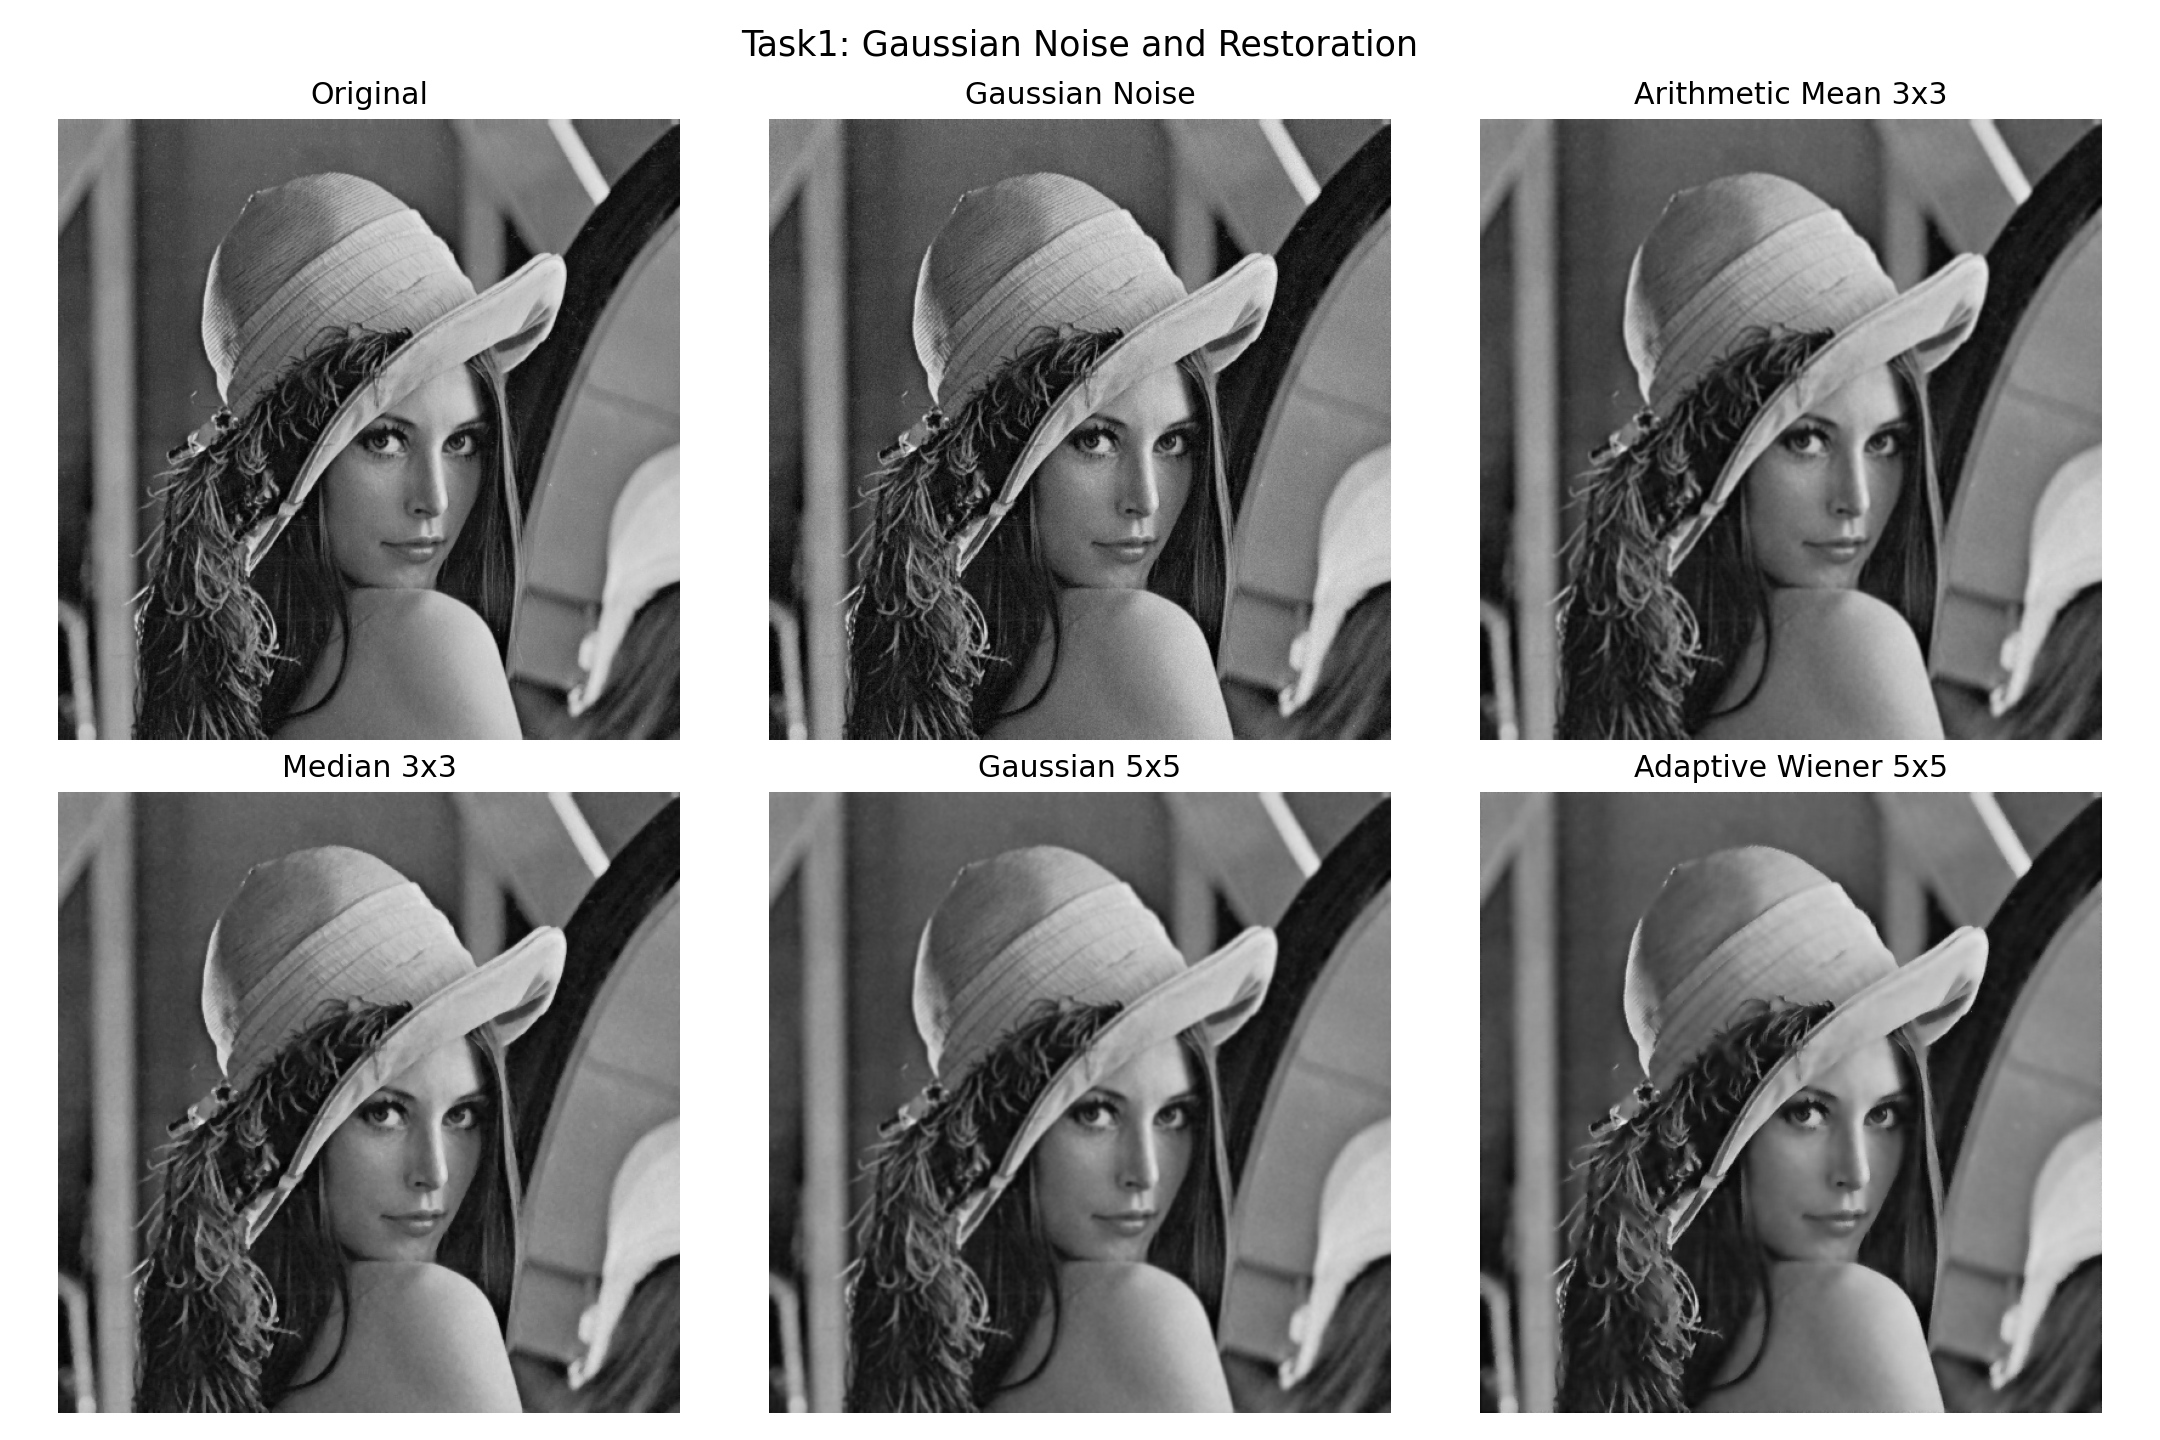
\includegraphics[width=\textwidth]{task1_overview.png}
  \caption{高斯噪声及多种恢复结果}
\end{figure}

\begin{table}[H]
\centering
\caption{任务1指标对比}
\begin{tabular}{lcc}
\toprule
方法 & MSE & PSNR(dB) \\
\midrule
Noisy & 19.942 & 35.133 \\
Arithmetic Mean 3x3 & 41.596 & 31.940 \\
Median 3x3 & 32.160 & 33.058 \\
Gaussian 5x5 & 44.003 & 31.696 \\
Adaptive Wiener 5x5 & 33.394 & 32.894 \\
\bottomrule
\end{tabular}
\end{table}

本实验中加入的高斯噪声强度相对较弱，因此噪声图本身的 PSNR 仍较高。恢复滤波器在抑制噪声的同时也引入了一定模糊，所以部分恢复图像的 PSNR 反而低于噪声图。这并不表示算法失效，而是说明当噪声较轻时，平滑带来的细节损失会在 MSE 指标上更显著。若从视觉效果看，自适应维纳滤波和中值滤波仍能在一定程度上改善噪点观感。

\subsection{任务2：椒盐噪声恢复}
\begin{figure}[H]
  \centering
  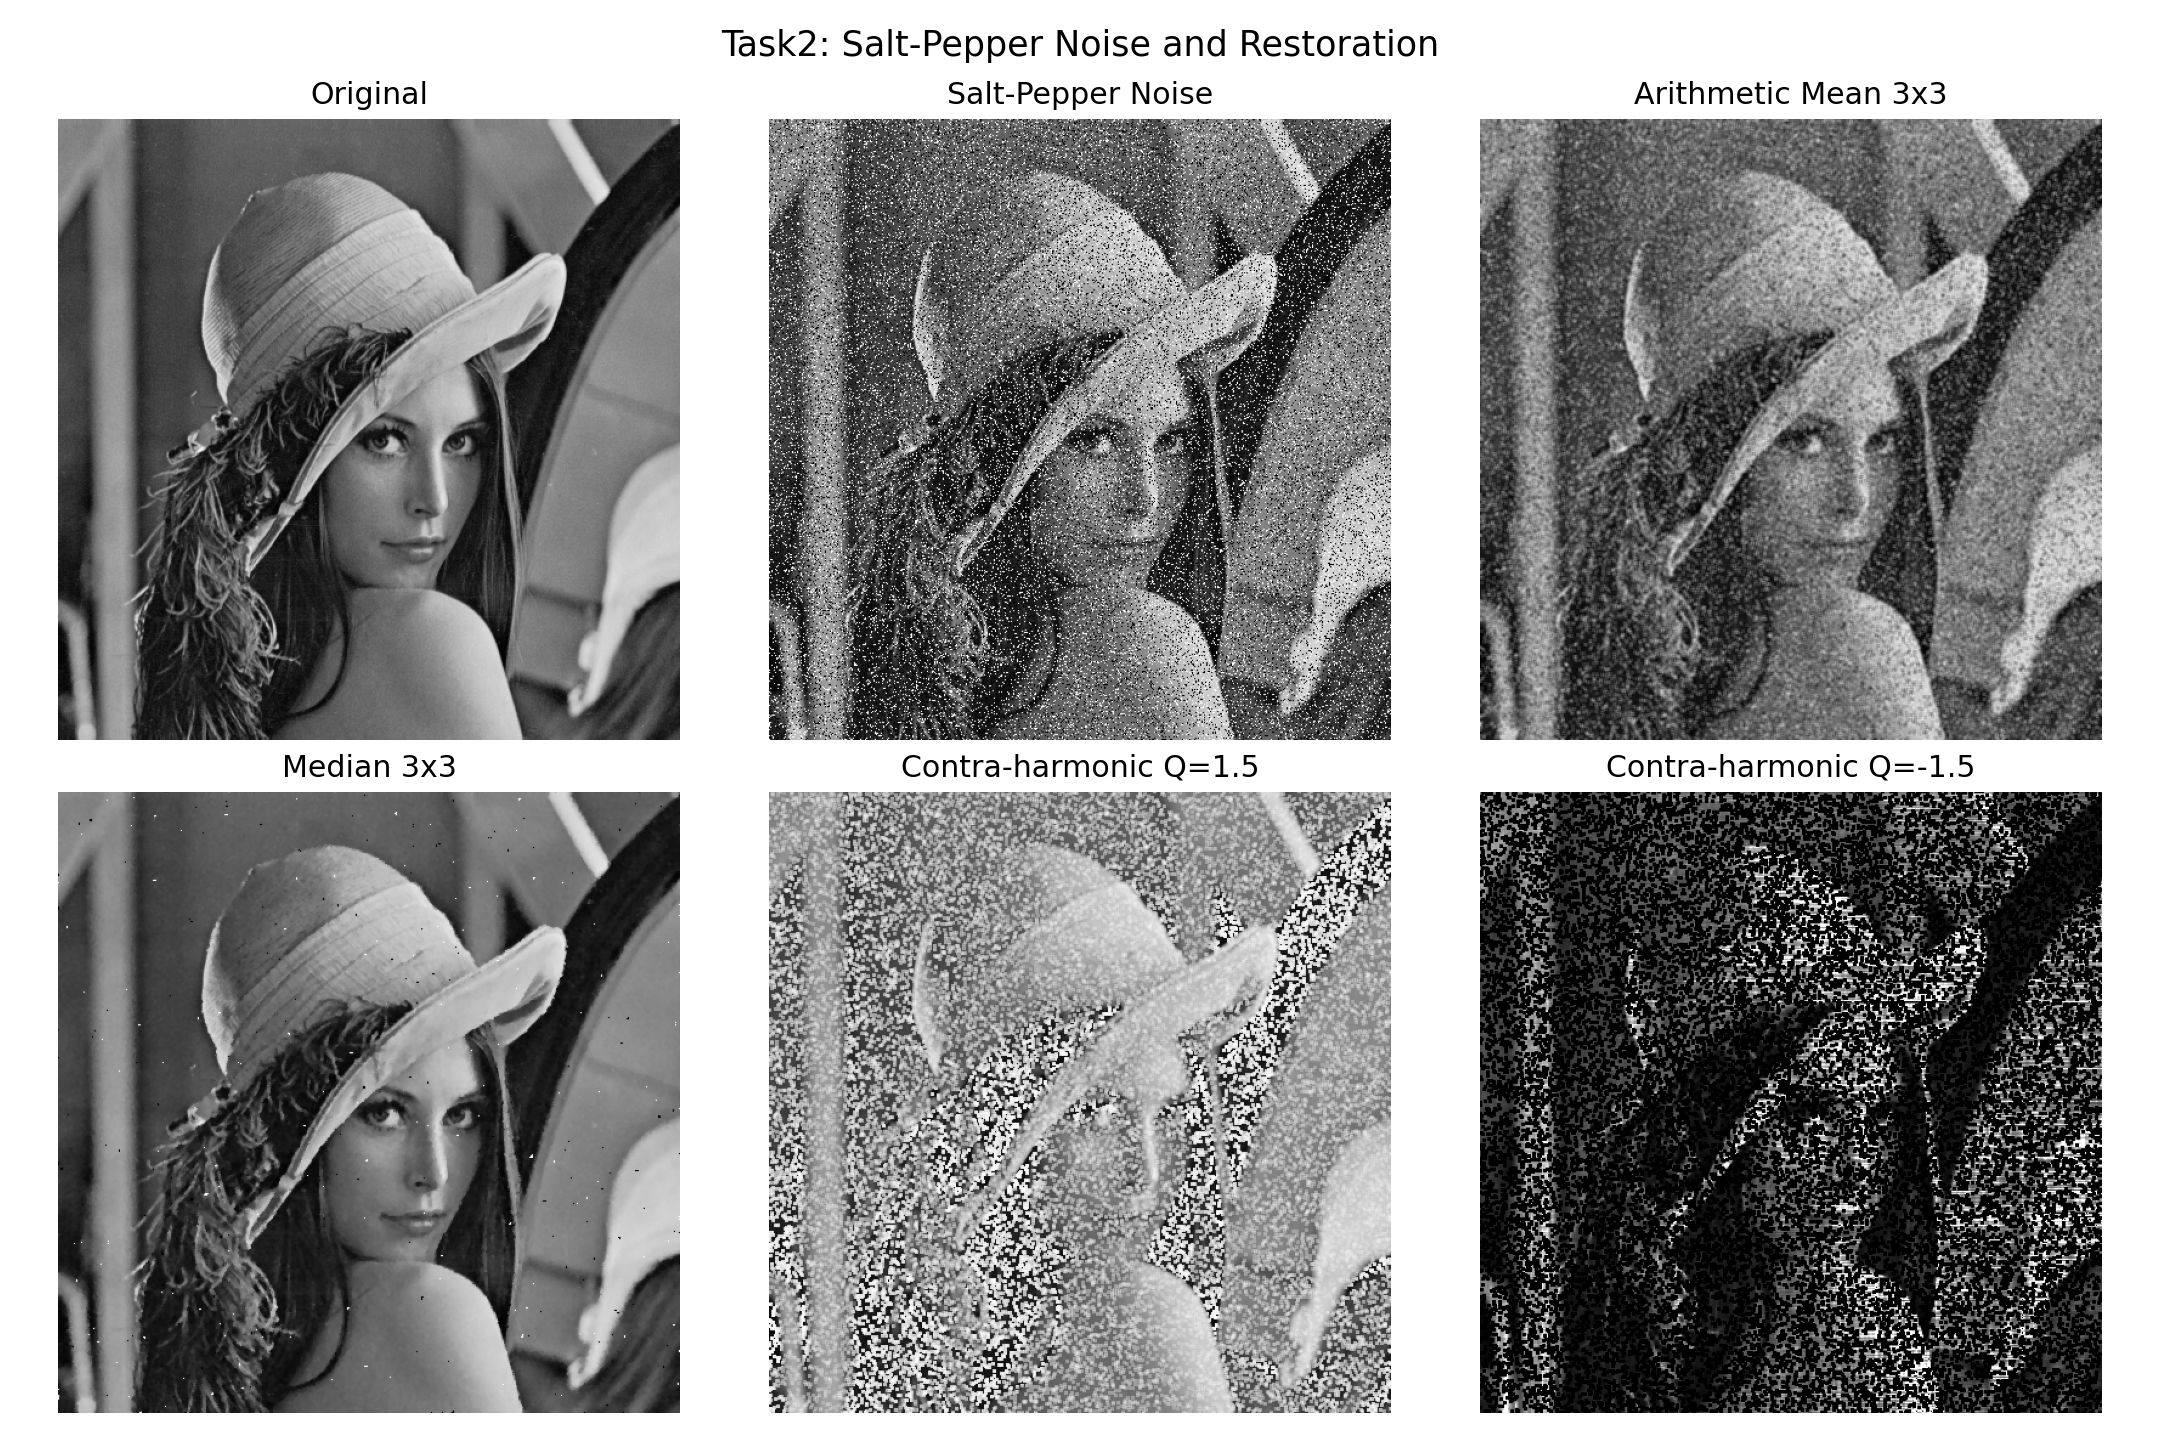
\includegraphics[width=\textwidth]{task2_overview.png}
  \caption{椒盐噪声及多种恢复结果}
\end{figure}

\begin{table}[H]
\centering
\caption{任务2指标对比}
\begin{tabular}{lcc}
\toprule
方法 & MSE & PSNR(dB) \\
\midrule
Noisy & 3964.802 & 12.149 \\
Arithmetic Mean 3x3 & 613.934 & 20.250 \\
Median 3x3 & 88.825 & 28.645 \\
Contra-harmonic Q=1.5 & 7371.855 & 9.455 \\
Contra-harmonic Q=-1.5 & 8166.385 & 9.011 \\
\bottomrule
\end{tabular}
\end{table}

从结果看，中值滤波对椒盐噪声恢复效果最好，说明它对脉冲型噪声最有针对性。反谐波滤波的表现较差，原因在于本实验同时存在较强的椒噪声和盐噪声，而单个 $Q$ 只能偏向抑制其中一种：
\begin{itemize}
  \item $Q>0$ 更偏向抑制椒噪声；
  \item $Q<0$ 更偏向抑制盐噪声。
\end{itemize}
当两者同时大量存在时，反谐波滤波难以兼顾，因此效果明显劣于中值滤波。

\subsection{任务3：运动模糊与维纳恢复}
\begin{figure}[H]
  \centering
  \begin{subfigure}{0.32\textwidth}
    \centering
    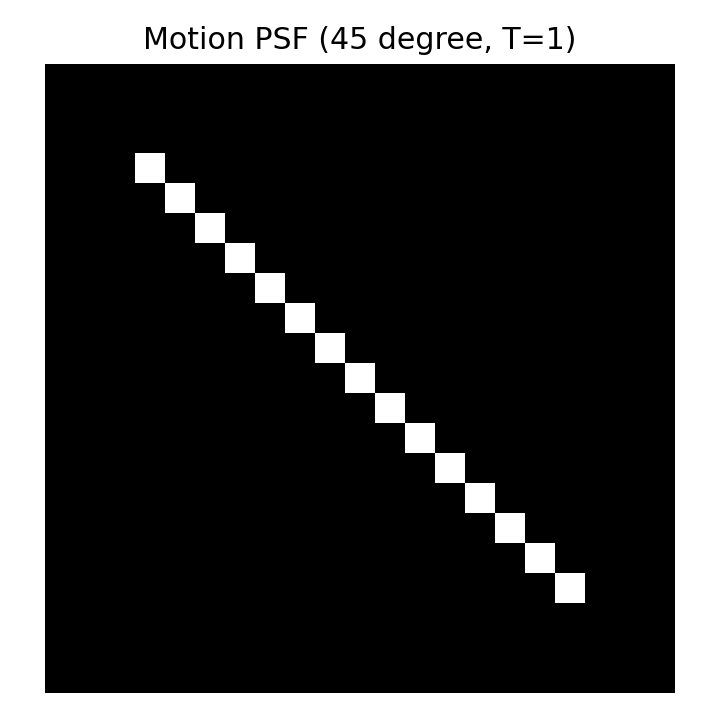
\includegraphics[width=\linewidth]{motion_psf.png}
    \caption{运动模糊 PSF}
  \end{subfigure}
  \begin{subfigure}{0.64\textwidth}
    \centering
    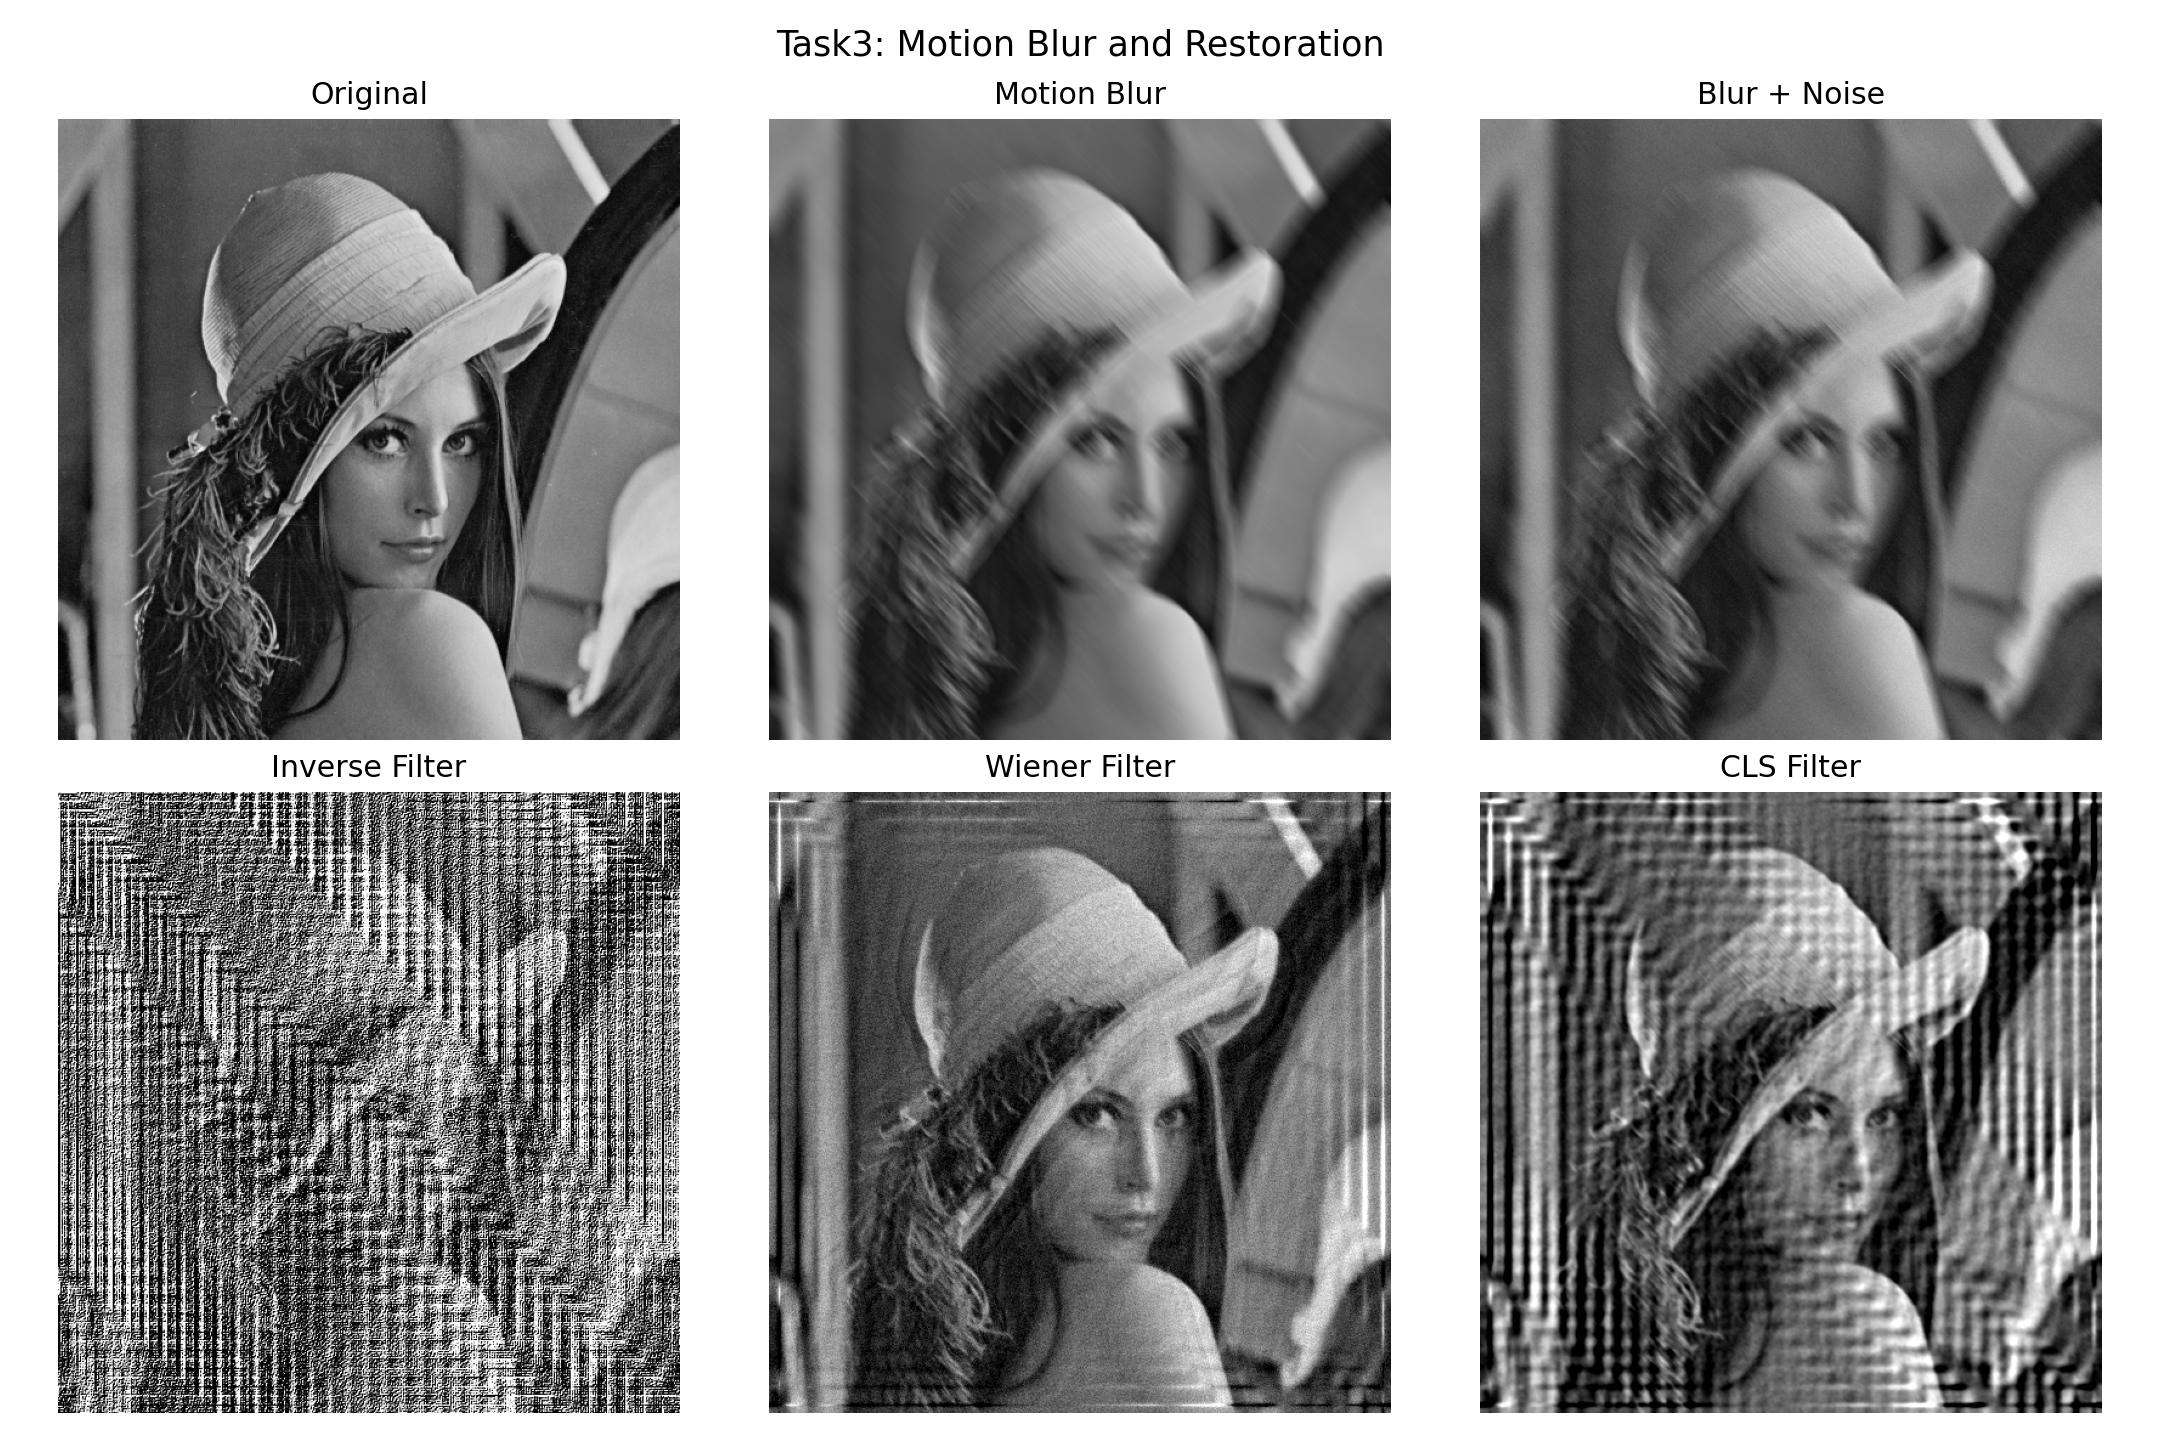
\includegraphics[width=\linewidth]{task3_overview.png}
    \caption{模糊、加噪与恢复结果}
  \end{subfigure}
  \caption{任务3结果}
\end{figure}

\begin{table}[H]
\centering
\caption{任务3指标对比}
\begin{tabular}{lcc}
\toprule
方法 & MSE & PSNR(dB) \\
\midrule
Blurred & 356.145 & 22.615 \\
Blurred + Gaussian Noise & 366.101 & 22.495 \\
Inverse Filter & 10536.218 & 7.904 \\
Wiener Filter & 526.118 & 20.920 \\
CLS Filter & 1385.695 & 16.714 \\
\bottomrule
\end{tabular}
\end{table}

逆滤波对噪声非常敏感，因此在模糊图加噪后恢复效果最差，出现了明显的条纹和伪影。维纳滤波显著优于逆滤波，说明在噪声存在时引入噪声约束十分必要。CLS 风格恢复相较逆滤波更稳定，但仍会产生较明显的规则性伪影，整体效果不如维纳滤波。

\subsection{综合分析}
\begin{table}[H]
\centering
\caption{不同恢复方法特点总结}
\begin{tabular}{p{3cm}p{5cm}p{5cm}}
\toprule
方法 & 优点 & 缺点 \\
\midrule
算术均值滤波 & 简单，对高斯噪声有一定抑制作用 & 易模糊边缘，对椒盐噪声不够鲁棒 \\
中值滤波 & 对椒盐噪声效果好，保边缘能力较强 & 对高斯噪声未必最优 \\
高斯滤波 & 适合高斯噪声，输出自然 & 会造成平滑模糊 \\
反谐波滤波 & 可针对椒噪声或盐噪声定向处理 & 参数 $Q$ 难兼顾两类噪声 \\
逆滤波 & 理论形式直接 & 极易放大噪声，稳定性差 \\
维纳滤波 & 能综合考虑噪声与模糊，恢复稳定 & 依赖噪声参数估计 \\
CLS 恢复 & 比逆滤波稳定，带有平滑约束 & 可能产生条纹和过平滑现象 \\
\bottomrule
\end{tabular}
\end{table}

\section{结论}
\begin{enumerate}
  \item 对高斯噪声，平滑类滤波器具有一定恢复能力，但当噪声较弱时，恢复结果未必在 PSNR 上优于噪声图。
  \item 对椒盐噪声，中值滤波最有效；反谐波滤波对 $Q$ 的选择高度敏感，且难以同时兼顾椒噪声和盐噪声。
  \item 对带噪运动模糊图像，逆滤波最不稳定，维纳滤波恢复效果最好，CLS 恢复介于两者之间。
  \item 图像恢复问题不仅取决于算法本身，也与噪声类型、强度和退化模型是否匹配密切相关。
\end{enumerate}

\section*{AI Report}
在\textbf{报告润色}方面，ChatGPT 主要用于辅助整理实验报告的文字表达，使实验步骤、结果分析与结论总结更加清晰、规范和完整。具体包括：将原始实验记录整理为正式书面语，对实验现象进行更规范的描述，对高斯噪声恢复、椒盐噪声去除、反谐波滤波中 $Q>0$ 与 $Q<0$ 的差异、运动模糊复原中逆滤波与维纳滤波效果差异等内容进行语言层面的归纳与表达优化，以及辅助生成符合实验报告风格的段落初稿。同时，AI 也用于辅助调整 LaTeX 文字内容的组织方式，例如章节说明、图表引导语、结果分析段落和总结性表述等。对于这些由 AI 辅助生成的文本内容，本人并未直接照搬，而是根据实验实际结果和课程要求进行了人工修改，以保证表述准确、逻辑连贯并符合本次实验的真实内容。

需要说明的是，本次实验中 AI 并不作为实验结果来源。所有退化图像、恢复图像、指标数据和最终结论均来源于本人实际运行代码后的实验输出；所有报告中的分析结论均建立在实验现象和人工判断基础之上。AI 在本实验中的作用主要体现在提高代码编写效率和优化文字表达质量，实验工作的主体设计、结果验证和最终责任仍由本人承担。

\vspace{0.5em}
\noindent\textbf{Main AI Tool Used:} ChatGPT

\vspace{0.5em}
\noindent\textbf{Example Prompts Used with ChatGPT:}
\begin{enumerate}
    \item ``Please help me implement Gaussian noise addition and compare arithmetic mean, median, Gaussian, and Wiener restoration filters in Python.''
    \item ``Help me write Python code to add salt-and-pepper noise to Lena and evaluate median filtering and contra-harmonic mean filtering with both positive and negative Q values.''
    \item ``Please implement motion blur degradation and restoration in Python, including inverse filtering, Wiener filtering, and constrained regularized restoration.''
    \item ``Check whether my image restoration code has potential issues in PSF construction, FFT-based restoration, parameter settings, and numerical stability.''
    \item ``Help me polish the wording of my lab report in Chinese so that the descriptions of noise restoration methods, experimental results, and conclusions sound more formal and academic.''
    \item ``Please rewrite my experimental observations into a clearer lab-report style and improve the logical flow of the analysis paragraphs.''
\end{enumerate}

\section*{附：编译与使用说明}
\begin{itemize}
  \item 建议在 Overleaf 选择 \textbf{XeLaTeX} 编译器。
  \item 上传本文件 \texttt{report\_hw6\_overleaf.tex} 与 \texttt{outputs/} 整个文件夹即可。
  \item 本文所有图片均直接来自 \texttt{outputs/task1\_gaussian\_noise}、\texttt{outputs/task2\_salt\_pepper} 和 \texttt{outputs/task3\_motion\_blur\_wiener}。
\end{itemize}

\end{document}
